\documentclass[11pt, A4paper]{article}
\usepackage[a4paper, total={7.2in, 10.5in}]{geometry}
\usepackage{tikz}
\usetikzlibrary{calc}
\usepackage{setspace}
\usepackage{graphicx}
\usepackage{amsmath}
\DeclareMathOperator\cis{cis}
\usepackage{pgfplots}
\graphicspath{ {./images/} }
\usepackage{bookmark}
\setcounter{tocdepth}{1}

\usepackage{mathptmx}

\hypersetup{
	colorlinks   = true, %Colours links instead of ugly boxes
	urlcolor     = blue, %Colour for external hyperlinks
	linkcolor    = black, %Colour of internal links
	citecolor   = red %Colour of citations
}

\newcommand{\tikzAngleOfLine}{\tikz@AngleOfLine}
\def\tikz@AngleOfLine(#1)(#2)#3{%
	\pgfmathanglebetweenpoints{%
		\pgfpointanchor{#1}{center}}{%
		\pgfpointanchor{#2}{center}}
	\pgfmathsetmacro{#3}{\pgfmathresult}%
}

\title{Further Pure Notes}
\author{Xingzhi Lu}
\date{For exams in 2025}

\begin{document}
	\maketitle
	\section{Further trigonometry}
	
	
	
	\section{Further calculus}
	
	
	
	
	\section{Further differential equations}
	
	
	
	
	
	\section{Coordinate systems}
	\subsection{Ellipse}
	\begin{itemize}
		\item $\dfrac{x^2}{a^2}+\dfrac{y^2}{b^2}=1$ \textbf{or}  $x=a\cos t$, $y=b\sin t$ ($o\leq t < 2\pi$)
	\end{itemize}
	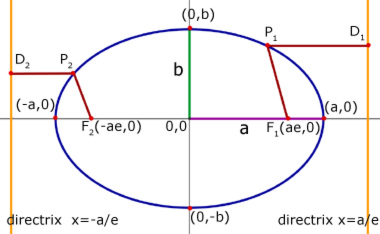
\includegraphics[width=0.25\textwidth]{ellipse}
	
	\subsection{Parabola}
	
	
	
	\subsection{Rectangular hyperbola}
	
	
	
	\section{Further vectors}
	\subsection{Finding areas of shapes}
	\begin{itemize}
		\item Area of triangle $\bigtriangleup ABC$ = $\dfrac{1}{2}|\overrightarrow{AB}\times\overrightarrow{AC}|$
		\item Area of parallelogram $ABCD$ = $|(b-a) \times (d-a)|=|(a\times b)+(b \times d) + (d \times a)|$ ($A$, $B$, $C$, $D$ have position vector $a$, $b$, $c$, $d$ respectively)
	\end{itemize}
	\subsection{Scalar triple product}
	\begin{itemize}
		\item Volume of parallelepiped = $a\cdot(b\times c)$ ($a$, $b$, $c$ = 3 different sides)
		\item Volume of tetrahedron $ABCD$ = $\dfrac{1}{6}|\overrightarrow{AD}\cdot(\overrightarrow{AB}\times\overrightarrow{AC})|$
	\end{itemize}
	\subsection{Straight lines}
	\subsubsection{Vector equation of line}
	\begin{itemize}
		\item $(\vec{r}-\vec{a})\times\vec{b}=0$
		\item $\vec{a}$ = position vector of a point on line, $\vec{b}$ = directional vector
	\end{itemize}
	\subsubsection{Direction cosines}
	For straight line $(r-a)\times b=0$, where $a=x\vec{i}+y\vec{j}+z\vec{k}$ and the line makes angle $\alpha$, $\beta$ and $\gamma$ with the positive $x$-, $y$- and $z$-axes respectively:
	\begin{itemize}
		\item $l=\cos\alpha = \dfrac{x}{|a|}$
		\item $m=\cos\beta = \dfrac{y}{|a|}$
		\item $n=\cos\gamma = \dfrac{z}{|a|}$
		\item $l^2+m^2+n^2=1$
	\end{itemize}
	
	\section{Further numerical methods}
	\section{Inequalities}

\end{document}